\subsection{A-Scan\label{sec:AScan}}
\todo{Hmmm, irgendwie war das jetzt doch ganz anders als letztes Mal und ich habe mir einfach etwas ausgedacht, das ich für sinnvoll erachtet habe...}
Die Tiefe der Löcher $d_\text{gemessen}$ im Acrylblock werden zunächst mit einer Schieblehre vermessen. Der A-Scan liefert im Anschluss daran Aufschluss über die Laufzeiten bis zur Stelle, an der der Schall reflektiert wird und zurück. Die nach nach 
\begin{align}
	s = \frac{1}{2} \cdot c_\text{Acryl} \cdot t
\end{align} mit $c_\text{Acryl} = \SI{2730}{\meter\per\second}$\footnote{\url{http://www.olympus-ims.com/de/ndt-tutorials/thickness-gage/appendices-velocities/}} berechneten Tiefen $d_\text{berechnet}$ sind alle etwas zu groß. Das liegt an der Übergangsschicht. Sie hat ungefähr die Dicke
\begin{align}
	d_\text{Übergangsschicht} = \frac{1}{11} \sum (d_\text{berechnet}-d_\text{gemessen}) \quad .
\end{align}
Die Messdaten führen zu Dicken der Übergangsschicht von
\begin{align}
	d_\text{Übergangsschicht, 1} = \SI{0.84}{\milli\meter} \\
	d_\text{Übergangsschicht, 2} = \SI{1.02}{\milli\meter}
\end{align}

	
Die wirkliche Tiefe ergibt sich damit nach
\begin{align}
	d_\text{korrigiert} =d_ \text{berechnet} - d_\text{Übergangsschicht}
\end{align}
Es ist immer die Tiefe der Lochoberkante gemeint. Die Werte für die beiden Messreihen sind in Tabelle~\ref{tab:werteA} dargestellt.


 \begin{figure}[h!]
 	\centering
 	\captionof{table}{Tiefen der Löcher in cm}
 	\begin{tabular}{ccc||ccc}
 		\multicolumn{3}{c}{Messung 1} & \multicolumn{3}{c}{Messung 2} \\
 		$d_\text{gemessen}$ & $d_\text{berechnet}$ & $d_\text{korrigiert}$ & $d_\text{gemessen}$ & $d_\text{berechnet}$ & $d_\text{korrigiert}$ \\
 		\hline
 		\input{build/tabelle_WerteA.txt}
 	\end{tabular}
 	\label{tab:werteA}
 \end{figure}
 
 
 
 
 
\subsection{B-Scan\label{sec:BScan}}
Zur einfacheren Beschreibung des Vorgehens wird nun definiert, dass die obere Kante in Abbildung \ref{fig:acrylblock} \emph{oben} sein soll und die in der Abbildung untere Kante \emph{unten}. \\
Es werden zwei B-Scans aufgenommen, einmal mit \emph{oben} oben und einmal mit \emph{unten} oben. Sie sind in Abbildung \ref{fig:BScan} dargestellt. Die Skala jeweils rechts kennzeichnet die Stärke des reflektierten Signals. Mit Hilfe des Bildbearbeitungsprogrammes \emph{gimp} und seiner \emph{Measure}-Funktion werden die Laufzeiten der Signale in den Graphiken gemessen. Genauer: Die Laufzeit des Signals von \emph{oben} bis zum jeweiligen Loch wird aus \ref{fig:oben} und die Laufzeit von \emph{unten} wird aus \ref{fig:unten} abgelesen. Abbildung \ref{fig:Schema} zeigt welcher Abstand dafür genau gewählt wird.
\begin{figure}[h!]
	\centering
	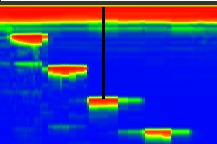
\includegraphics[width=0.35\textwidth]{Schema.png}
	\caption{Die senkrechte schwarze Linie kennzeichnet welcher Abstand im B-Scan zur Bestimmung der Laufzeit des Signals verwendet wird.}
	\label{fig:Schema}
\end{figure} \\
\todo[color = red, inline]{Hier dachte ich: OK, bei rot ist immer irgendwie Luft, bzw. ganz oben ist der rote Balken halt der Übergang zwischen Sonde und Glas. Also messe ich von der Unterkante des roten Balkens (weil da ja das Glas erst losgeht) bis zur Oberkante des jeweiligen Lochs. Dann sind die Werte aber viel zu klein. Von der Oberkante weg passts ganz gut. Kannst du das erklären?}
\todo{Ja, ich weiß, die Scans sind sehr klein, aber für ein Protokoll ist das sonst zu viel Tintenverschwendung.}
\begin{figure}[h!]
	\centering
	\begin{subfigure}{.45\textwidth}
		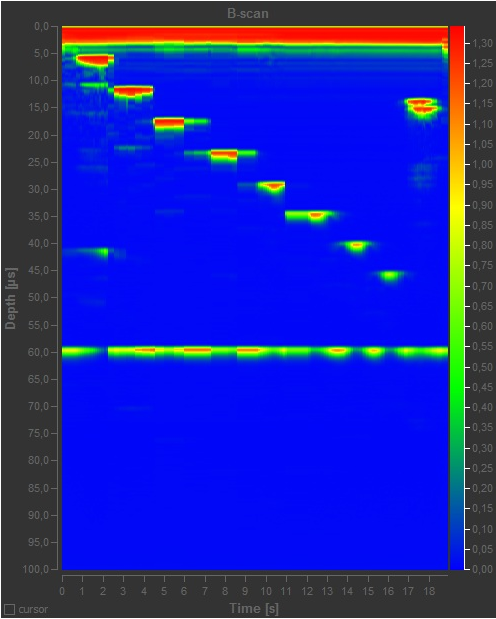
\includegraphics[width=\textwidth]{oben.png}
		\caption{von \emph{oben}}
		\label{fig:oben}
	\end{subfigure}
	\begin{subfigure}{.45\textwidth}
		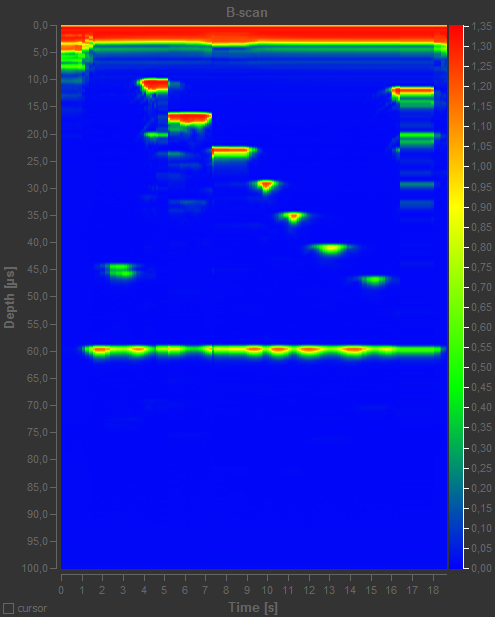
\includegraphics[width=\textwidth]{unten.png}
		\caption{von \emph{unten}}
		\label{fig:unten}
	\end{subfigure}
	\caption{Aufgenommene B-Scans}
	\label{fig:BScan}
\end{figure}
Das Computerprogramm misst die Abstände in Pixeln. Zur Umrechnung in Sekunden wird mit der linken Skala der Maßstab
\begin{align}
	\SI{100}{\micro\second} \ \widehat{=} \ \SI{544}{Pixel}
\end{align}
bestimmt. Die so bestimmten Laufzeiten stehen in Tabelle \ref{tab:Zeit}. Loch 10 müsste im Scan \ref{fig:unten} rechts unten zu sehen sein. Wie an dem verschmierten Signal darüber von Loch 11 zu sehen ist, ist die Aufnahme dort nicht optimal, sodass kein Wert gemessen werden kann und der Wert 0 eingetragen wird.
\begin{table}
    \centering
    \caption{Aus den B-Scans bestimmte Laufzeiten in Pixeln $\tilde{t}$ und umgerechnete Laufzeiten $t$}
    \label{tab:Zeit}
    \sisetup{parse-numbers=false}
    \begin{tabular}{
	S[table-format=3.0]
	S[table-format=2.2]
	S[table-format=3.0]
	S[table-format=2.2]
	}
	\toprule
	{$\tilde{t}_\text{oben}$ in \si{Pixel}}		& {$t_\text{oben}$ in \si{\micro\second}}		& 
	{$\tilde{t}_\text{unten}$ in \si{Pixel}}		& {$t_\text{unten}$ in \si{\micro\second}}		\\ 
	\midrule
    80  & 14.73 & 238 & 43.83 \\
73  & 13.44 & 245 & 45.12 \\
247 & 45.49 & 54  & 9.94  \\
216 & 39.78 & 88  & 16.21 \\
186 & 34.25 & 123 & 22.65 \\
156 & 28.73 & 156 & 28.73 \\
125 & 23.02 & 189 & 34.81 \\
92  & 16.94 & 221 & 40.70 \\
60  & 11.05 & 253 & 46.59 \\
29  & 5.34  & 0   & 0.00  \\
224 & 41.25 & 63  & 11.60 \\

    \bottomrule
    \end{tabular}
    \end{table}
 \\
Mit der in \ref{sec:AScan} bestimmten Schallgeschwindigkeit $c$ kann nun der Abstand der Löcher nach \emph{oben}
\begin{align}
	s_\text{oben} = c \cdot t_\text{oben} \ ,
\end{align}
bzw. nach \emph{unten}
\begin{align}
	s_\text{unten} = c \cdot t_\text{unten} \ ,
\end{align}
berechnet werden. Die Vermessung des Quaders ergibt eine Gesamthöhe von
\begin{align}
	h = \SI{80.20}{\milli\meter} \ ,
\end{align}
sodass auch der Durchmesser der Löcher
\begin{align}
	d = h - s_\text{oben} - s_\text{unten}
\end{align}
bestimmt werden kann. Die so berechneten Werte werden in Tabelle \ref{tab:ObenGanz} mit den gemessenen Werten verglichen.
\begin{table}
    \centering
    \caption{Berechnete Abstände der Löcher zum oberen Rand $s_\text{oben}$ und zum unteren Rand $s_\text{unten}$, die daraus bestimmte Dicke der Löcher $d$ und jeweils dazu die gemessenen Werte $\tilde{x}_\text{gem.}$. Alle Werte in \si{\milli\meter}.}
    \label{tab:ObenGanz}
    \sisetup{parse-numbers=false}
    \begin{tabular}{
	S[table-format=2.2]
	S[table-format=2.2]
	S[table-format=2.2]
	S[table-format=2.2]
	S[table-format=2.2]
	S[table-format=2.2]
	}
	\toprule
	{$s_\text{oben}$}		& {$\tilde{s}_\text{oben}$}		& 
	{$s_\text{unten}$}		& {$\tilde{s}_\text{unten}$}		& 
	{$d$}		& {$\tilde{d}$}		\\ 
	\midrule
    20.04 & 20.55 & 59.61 & 60.00 & 0.55  & -0.35 \\
18.28 & 18.25 & 61.36 & 61.70 & 0.55  & 0.25  \\
61.86 & 61.30 & 13.52 & 13.10 & 4.81  & 5.80  \\
54.10 & 54.20 & 22.04 & 21.70 & 4.06  & 4.30  \\
46.59 & 46.70 & 30.81 & 29.95 & 2.81  & 3.55  \\
39.07 & 38.95 & 39.07 & 38.95 & 2.06  & 2.30  \\
31.31 & 30.80 & 47.34 & 46.50 & 1.56  & 2.90  \\
23.04 & 23.40 & 55.35 & 54.75 & 1.81  & 2.05  \\
15.03 & 15.40 & 63.37 & 62.90 & 1.81  & 1.90  \\
7.26  & 7.05  & 0.00  & 70.95 & 72.94 & 2.20  \\
56.10 & 55.50 & 15.78 & 14.90 & 8.32  & 9.80  \\

    \bottomrule
    \end{tabular}
    \end{table}

\clearpage
\subsection{TM-Scan}
Zunächst wird mit einem A-Scan die Laufzeit eines Ultraschall-Signals im Ruhezustand bestimmt. Sie beträgt
\begin{align}
	t = \SI{58.3}{\micro\second} \ .
\end{align}
Mit der Schallgeschwindigkeit in Wasser
\begin{align}
	c_\text{Wasser} = \SI{1484}{\meter\per\second}
\end{align}
\todo{Quelle} wird die Wasserhöhe
\begin{align}
	h_\text{Herz} = \SI{43.3}{\milli\meter}

\end{align}
bestimmt. Während des Pumpens, wird ein TM-Scan durchgeführt, der in Abbildung \ref{fig:Herz} zu sehen ist. Daraus wird abgelesen, dass das Herz mit einer Frequenz von
\begin{align}
	\nu = \frac{6}{16}\si{\hertz} = \SI{0.375}{\hertz}
\end{align}
\grqq schlägt\grqq.
\begin{figure}[h!]
	\centering
	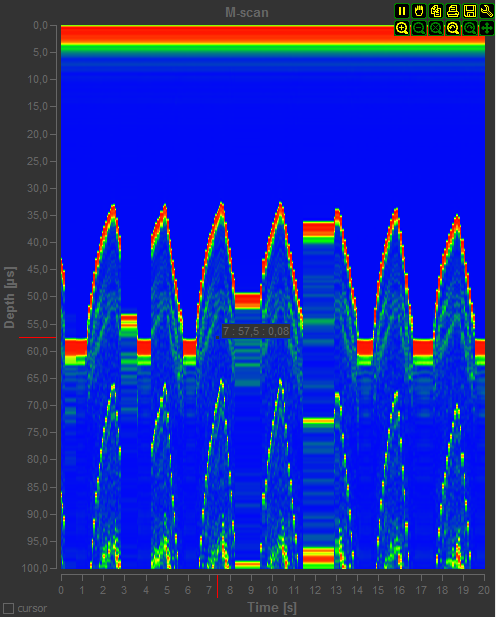
\includegraphics[width=0.6\textwidth]{TimeScan.png}
	\caption{TM-Scan eines pulsierenden Herz-Modells}
	\label{fig:Herz}
\end{figure} \\
Als Diastole wird die Phase bezeichnet, in der sich das Herz entspannt und dadurch mit Blut füllt. Im TM-Scan sind das die abfallenden Flanken der Peaks, an den Tiefpunkten ist das Blutvolumen im Herzmodell maximal. Dieses Volumen wird enddiastolisches Herzvolumen EDV genannt. In diesem Fall, ist das das Volumen eines Zylinders mit Höhe $h_\text{Herz}$ und Durchmesser
\begin{align}
        d_\text{Herz} = \SI{49.45}{\milli\meter} \ .
\end{align}
Während der Systole kontrahiert das Herz und pumpt das Blut in den Körper, die Kurve im TM-Scan steigt. Das Maximum der Kurve kennzeichnet den Zeitpunkt des endsystolischen Volumens ESV, es ist das kleinste Blutvolumen während eines Zyklusses. Das ESV wird als der Zylinder mit $h_\text{Herz}$ und $d_\text{Herz}$, reduziert durch das Volumen eines Kugelsegments mit Durchmesser $d_\text{Herz}$ und Höhe $a$ genähert. In Formeln ausgdrückt bedeutet das
\begin{align}
	EDV &= \pi \frac{d^2_\text{Herz}}{4} h_\text{Herz} \\
	ESV &= \pi \frac{d^2_\text{Herz}}{4} h_\text{Herz} - \frac{a}{3} \pi (3d_\text{Herz}^2 + a^2) \ .
\end{align}
Das Herzvolumen HZV ist definiert als
\begin{align}
	\text{HZV} &= (\text{EDV} - \text{ESV}) \cdot \nu \\
	&= \frac{a}{3} \pi (\frac{3}{4}d_\text{Herz}^2 + a^2) \cdot \nu \ .
\end{align}
Aus dem TM-Scan werden die Laufzeiten der Schallwelle an den Minima und Maxima mit der in Kapitel \ref{sec:BScan} beschriebenen Methode extrahiert. Sie sind in Tabelle \ref{tab:HerzZeit} aufgetragen. Die Werte der Maxima und der Minima werden jeweils gemittelt und mit der Differenz der beiden $t_\text{Herz}$ kann die Höhe $a$ bestimmt werden
\begin{align}
	a &= \frac{1}{2}c_\text{Wasser}t_\text{Herz} \\
	&= \SI{17.2+-0.4}{\milli\meter}
 \ .
\end{align}
Damit kann das Herzvolumen bestimmt werden
\begin{align}
	\text{HZV} = \SI{14.4+-0.4}{\centi\meter\cubed}
 \ .
\end{align}
\begin{table}
    \centering
    \caption{Aus dem TM-Scan bestimmte Laufzeiten in Pixeln $\tilde{t}$ und umgerechnete Laufzeiten $t$}
    \label{tab:ZeitHerz}
    \sisetup{parse-numbers=false}
    \begin{tabular}{
	S[table-format=3.0]
	S[table-format=2.2]
	S[table-format=3.0]
	S[table-format=2.2]
	}
	\toprule
	{$\tilde{t}_{max}$ in \si{Pixel}}		& {$t_{max}$ in \si{\micro\second}}		& 
	{$\tilde{t}_{min}$ in \si{Pixel}}		& {$t_{min}$ in \si{\micro\second}}		\\ 
	\midrule
    179 & 32.97 & 315 & 58.01 \\
179 & 32.97 & 314 & 57.83 \\
179 & 32.97 & 315 & 58.01 \\
179 & 32.97 & 268 & 49.36 \\
185 & 34.07 & 315 & 58.01 \\
185 & 34.07 & 316 & 58.20 \\
191 & 35.17 & 315 & 58.01 \\

    \bottomrule
    \end{tabular}
    \end{table}

